\documentclass[11pt]{ctexart}

% Self-contained NeurIPS-like report layout.
% Overleaf: set compiler to XeLaTeX.
\usepackage[a4paper,margin=1in]{geometry}
\usepackage{amsmath,amssymb}
\usepackage{booktabs}
\usepackage{graphicx}
\usepackage{caption}
\usepackage{subcaption}
\usepackage{enumitem}
\usepackage{array}
\usepackage{xcolor}
\usepackage{hyperref}
\usepackage{url}
\usepackage{fancyhdr}
\usepackage{titlesec}

\hypersetup{
  colorlinks=true,
  linkcolor=blue!55!black,
  citecolor=blue!55!black,
  urlcolor=blue!55!black
}

\pagestyle{fancy}
\fancyhf{}
\lhead{HW3 题目二：LeRobot ACT 跨环境泛化}
\rhead{\thepage}
\renewcommand{\headrulewidth}{0.4pt}

\titleformat{\section}{\large\bfseries}{\thesection}{0.6em}{}
\titleformat{\subsection}{\normalsize\bfseries}{\thesubsection}{0.6em}{}
\setlist[itemize]{leftmargin=1.2em}
\setlist[enumerate]{leftmargin=1.4em}

\newcommand{\methodA}{ACT-A}
\newcommand{\methodABC}{ACT-ABC}
\newcommand{\actlone}{Action L1}

\title{\bfseries 基于 LeRobot 的 ACT 策略跨环境泛化挑战}
\author{
  姓名：\textbf{TODO: 填写姓名} \\
  学号：\textbf{TODO: 填写学号} \\
  课程：深度学习与空间智能
}
\date{\today}

\begin{document}
\maketitle

\begin{center}
\begin{tabular}{ll}
\toprule
项目代码仓库 & \url{https://github.com/Zhan-xing-pz/CS60003-HW3} \\
模型权重下载 & \url{TODO: https://pan.baidu.com/s/<share-id>} \\
实验目录 & \texttt{/data2/pz/homework/hw3} \\
\bottomrule
\end{tabular}
\end{center}

\begin{abstract}
本文围绕 CALVIN 多环境数据集上的视觉-动作模仿学习问题，使用 LeRobot 框架中的 Action Chunking with Transformers (ACT) 策略研究跨环境泛化能力。实验比较了两种训练设置：仅使用环境 A 数据训练的基础策略 \methodA{}，以及混合环境 A/B/C 数据训练的多环境联合策略 \methodABC{}。两个模型采用完全一致的 ACT 网络结构与训练超参数，并只使用训练环境内部划分的 validation split 选择最优 checkpoint；环境 D 仅用于最终 zero-shot 测试。实验结果显示，\methodABC{} 在验证集和未见过的环境 D 上均显著优于 \methodA{}：在 D 环境的 200-batch 离线评估中，\methodABC{} 的 mean \actlone{} 为 0.4471，低于 \methodA{} 的 0.4963。该现象表明，多环境联合训练能够缓解视觉分布偏移导致的策略退化；同时，ACT 的动作分块机制通过预测连续动作片段提供了时间一致性，有助于在跨环境视觉偏移下保持更稳定的动作输出。
\end{abstract}

\section{任务背景}
机器人模仿学习通常需要从视觉观测、机器人状态与专家动作序列中学习闭环控制策略。然而，当训练和测试环境在背景纹理、光照、物体摆放或相机观测分布上发生偏移时，视觉策略容易出现跨环境泛化退化。本实验关注的核心问题是：仅在单一环境中训练的 ACT 策略能否泛化到未见过环境，以及混合多个训练环境是否能提升 zero-shot 跨环境表现。

题目要求完成三个部分：首先，基于 LeRobot 框架中的 ACT 算法，仅使用 CALVIN 环境 A 训练基础视觉-动作策略；其次，将环境 A/B/C 数据混合，在相同 ACT 网络结构和超参数下训练多环境联合模型；最后，将两个模型部署到完全未见过的环境 D 中进行 zero-shot 测试，并比较成功率或动作误差。由于本次提供的 D 环境离线数据不包含真实任务完成信号，本文使用 mean \actlone{} 作为主要评估指标，success rate 保持空值。

\section{数据集描述}
实验使用 Hugging Face 上的 \texttt{huiwon/calvin\_task\_ABC\_D} 数据集，并转换为 LeRobot v3.0 数据格式。CALVIN 数据集包含多个视觉环境，每个环境提供机器人状态、RGB 观测和专家动作。本文将环境 A 作为单环境训练集，将环境 A/B/C 合并为联合训练集，并将环境 D 完全保留为最终 zero-shot 测试环境。

训练和验证不使用环境 D。对于 \methodA{}，从环境 A 中按 episode 做 90\%/10\% 划分；对于 \methodABC{}，分别从 A、B、C 各自按 90\%/10\% 划分后混合得到训练与验证集合。这样可以保证 best checkpoint 的选择只依赖训练域内部的 validation \actlone{}，避免用测试环境 D 调参。

\begin{table}[t]
\centering
\caption{数据划分统计。frames 为 LeRobot 数据中的逐帧样本数。}
\label{tab:data_split}
\begin{tabular}{lrrrrr}
\toprule
设置 & Train Episodes & Valid Episodes & Train Frames & Valid Frames & Total Frames \\
\midrule
\methodA{}: A-only & 4021 & 447 & 240772 & 26910 & 267682 \\
\methodABC{}: A/B/C joint & 12062 & 1341 & 723960 & 80410 & 804370 \\
D zero-shot eval & -- & -- & -- & -- & 267373 \\
\bottomrule
\end{tabular}
\end{table}

\section{方法原理}
ACT 是一种面向精细操作任务的轻量级模仿学习策略。根据 LeRobot 文档，ACT 使用视觉骨干网络处理多视角图像，通过 Transformer 编码器融合图像特征、机器人状态和潜变量，并由 Transformer 解码器一次性预测未来 $k$ 个动作组成的动作块。本文设定 chunk size 为 16，即模型每次输出 16 步未来动作。

动作分块机制的关键优势在于时间一致性。普通逐步预测策略需要在每一帧都独立决定下一动作，因而容易对视觉噪声或单帧分布偏移敏感；ACT 通过输出连续动作序列，使策略在短时间窗口内具有更平滑的控制意图。面对环境 D 中未见过的视觉外观时，这种机制有助于降低短时动作抖动，但如果视觉编码器只见过单一环境，仍可能把背景或光照变化误解释为状态变化。因此，本文假设 A/B/C 联合训练能够提升视觉表征的环境不变性，并与 ACT 的动作分块机制互补。

\section{实验设置}
两个模型除数据来源不同外，网络结构、优化器、训练步数、batch size、学习率和 checkpoint 选择逻辑完全一致。训练总步数设置为 30000，每 1000 step 保存候选 checkpoint，并在训练环境 validation split 上评估 50 batches 的 mean \actlone{}。若当前 checkpoint 的 validation \actlone{} 低于历史最优，则更新 \texttt{checkpoints/best/pretrained\_model}；否则丢弃该候选 checkpoint。最终只使用 validation-best checkpoint 在 D 环境做一次 200-batch zero-shot 评估。

\begin{table}[t]
\centering
\caption{模型结构与训练超参数。两个模型完全一致，仅训练数据不同。}
\label{tab:hparams}
\begin{tabular}{ll}
\toprule
项目 & 设置 \\
\midrule
Framework & LeRobot ACT \\
Policy Type & \texttt{act} \\
Vision Backbone & ResNet-18 style visual encoder in ACT \\
Transformer Hidden Dim & 256 \\
Transformer Encoder Layers & 4 \\
Transformer Decoder Layers & 4 \\
Attention Heads & 8 \\
Dropout & 0.1 \\
Action Chunk Size & 16 \\
Action Steps & 16 \\
Batch Size & 64 \\
Training Steps & 30000 \\
Optimizer & AdamW \\
Learning Rate & $1.0\times 10^{-4}$ \\
Weight Decay & $1.0\times 10^{-6}$ \\
Loss Function & L1 imitation loss \\
Checkpoint Frequency & 1000 steps \\
Validation per Checkpoint & 50 batches \\
Final D Evaluation & 200 batches \\
WandB/SwanLab & TODO: 上传本地 CSV/PNG 后替换为平台导出图 \\
\bottomrule
\end{tabular}
\end{table}

\section{实验结果}
\subsection{训练过程与验证曲线}
图~\ref{fig:train_valid} 展示了两个模型的训练 loss 和 validation \actlone{} 曲线。可以观察到，训练 loss 随训练步数整体下降，但 validation \actlone{} 并不单调下降，而是存在明显波动。这说明仅看训练 loss 容易误判模型泛化能力，必须基于 validation 指标选择 checkpoint。

\begin{figure}[t]
\centering
\begin{subfigure}{0.48\linewidth}
\centering
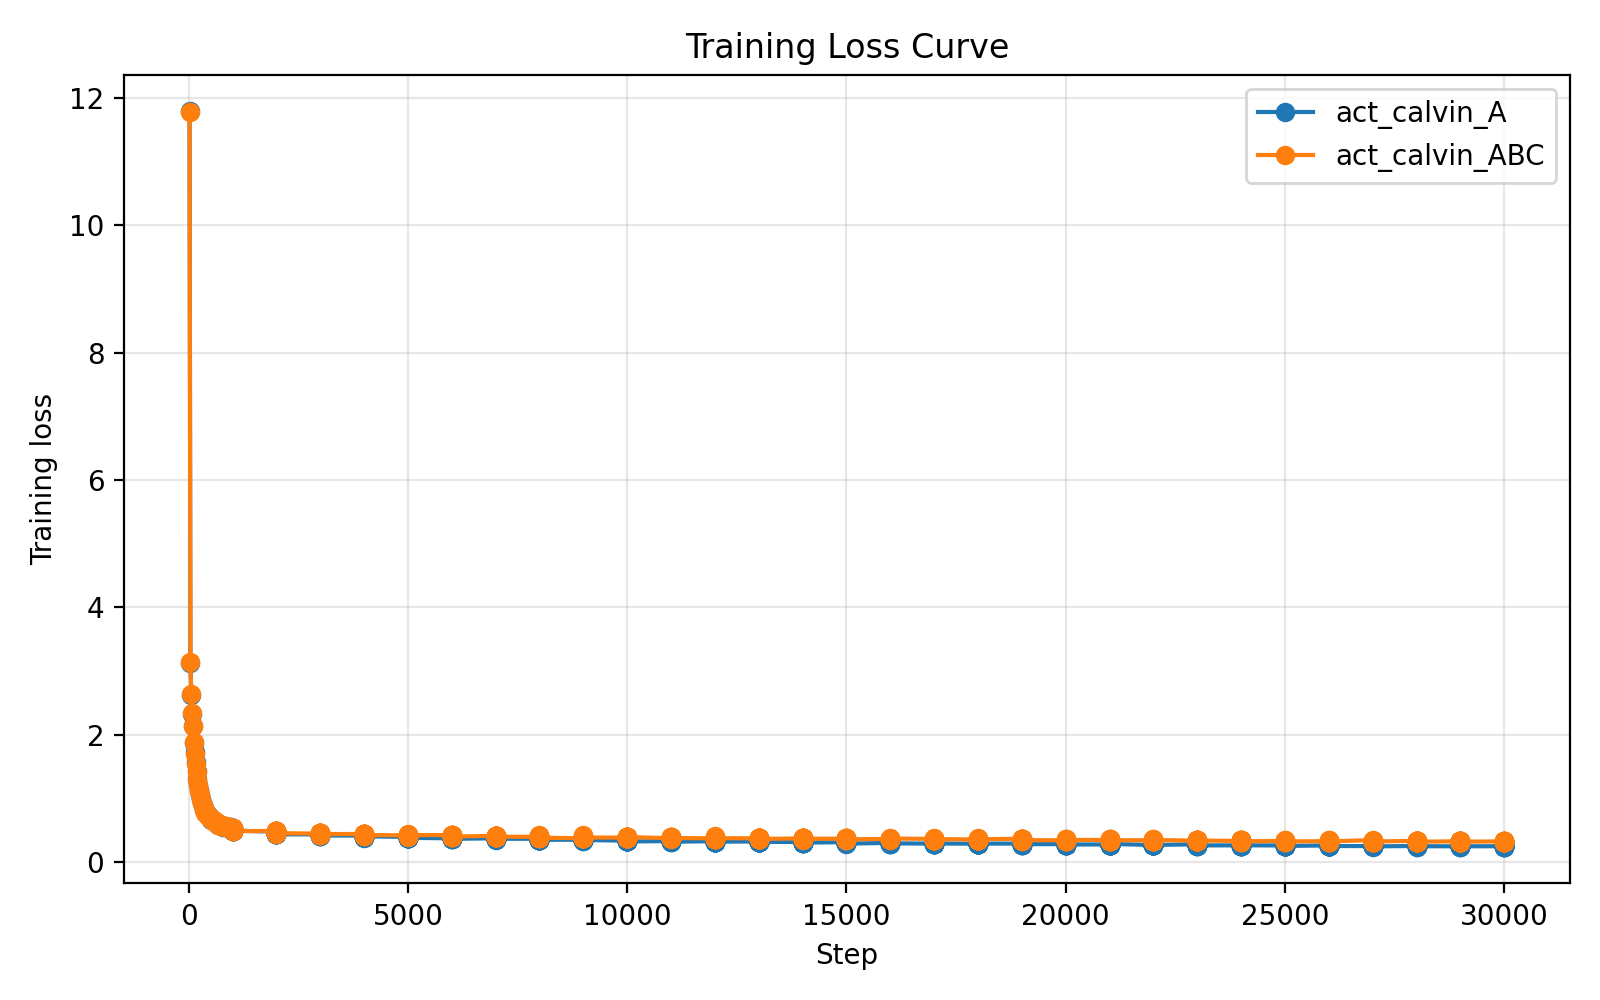
\includegraphics[width=\linewidth]{figures/train_loss_curve.png}
\caption{训练 loss 曲线}
\end{subfigure}
\hfill
\begin{subfigure}{0.48\linewidth}
\centering
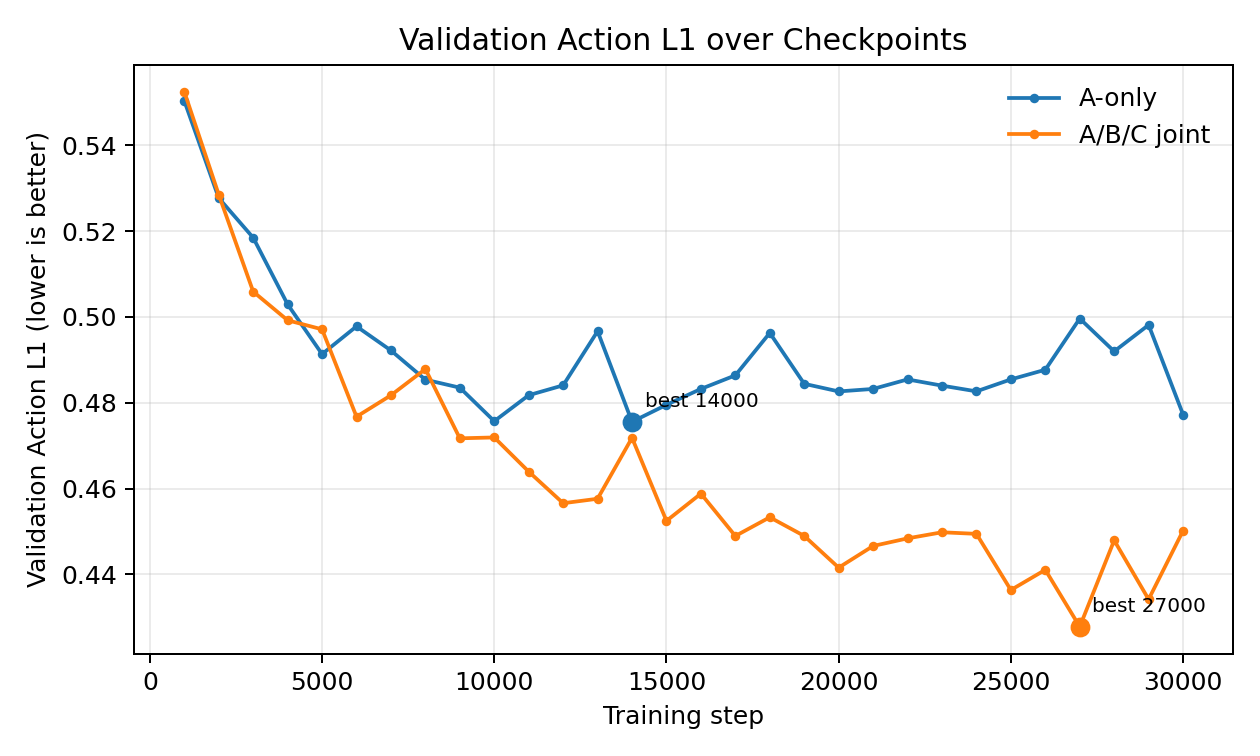
\includegraphics[width=\linewidth]{figures/valid_action_l1_curve.png}
\caption{Validation \actlone{} 曲线}
\end{subfigure}
\caption{训练过程可视化。当前图由本地 CSV 日志导出；若最终提交严格要求 WandB/SwanLab，可将同一 CSV 上传至平台后导出替换。}
\label{fig:train_valid}
\end{figure}

从 validation 曲线看，\methodA{} 在 14000 step 达到最优 validation \actlone{} 0.4755，之后较长时间没有稳定改进，表现出平台期或过拟合迹象。\methodABC{} 则在更长训练后仍能受益，于 27000 step 达到最优 validation \actlone{} 0.4278。二者的差异说明，多环境数据不仅提高了最终精度，也改变了训练动态：多环境模型需要更长时间学习更复杂的视觉变化，但最终获得更稳健的表征。

\subsection{Zero-shot D 环境评估}
表~\ref{tab:final_metrics} 给出了两个 validation-best 模型在 D 环境上的最终 zero-shot 评估结果。由于 D 环境离线数据没有任务完成信号，success rate 为空；本文主要比较 mean \actlone{} 和 std \actlone{}。

\begin{table}[t]
\centering
\caption{最终 validation-best checkpoint 与 D 环境 zero-shot 指标。}
\label{tab:final_metrics}
\begin{tabular}{lrrrrr}
\toprule
模型 & Best Step & Valid \actlone{} & D Mean \actlone{} & D Std \actlone{} & Eval Batches \\
\midrule
\methodA{} & 14000 & 0.475544 & 0.496255 & 0.147399 & 200 \\
\methodABC{} & 27000 & 0.427793 & 0.447098 & 0.127290 & 200 \\
\bottomrule
\end{tabular}
\end{table}

\begin{figure}[t]
\centering
\begin{subfigure}{0.48\linewidth}
\centering
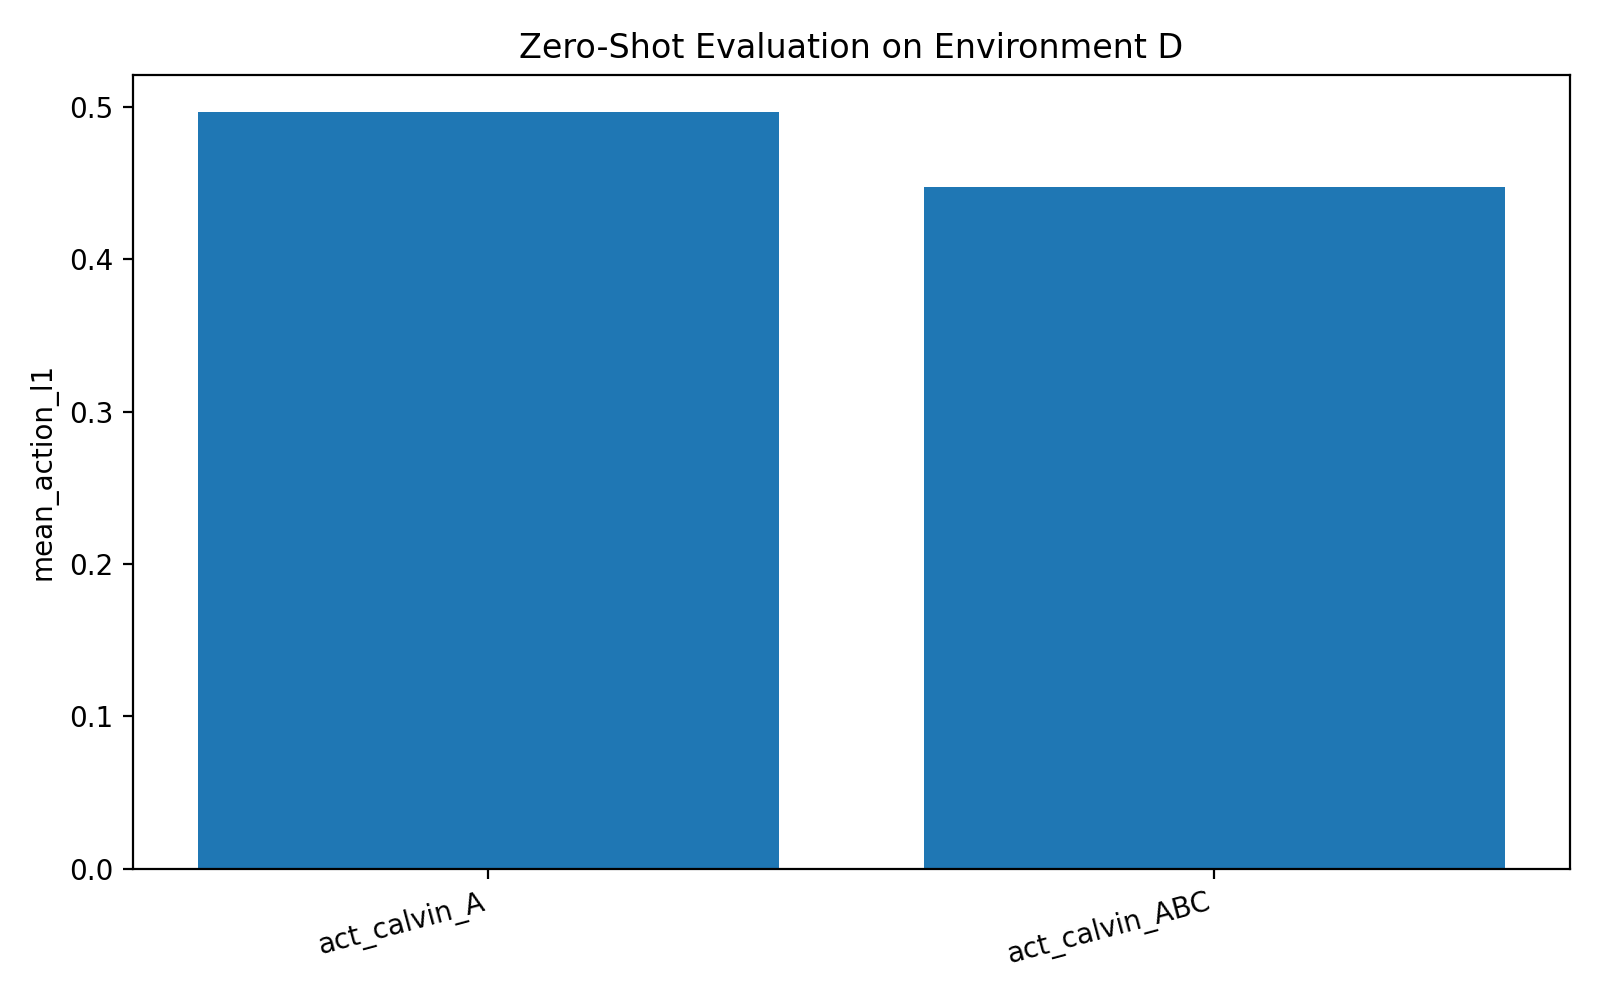
\includegraphics[width=\linewidth]{figures/eval_D_bar.png}
\caption{D 环境 mean \actlone{} 对比}
\end{subfigure}
\hfill
\begin{subfigure}{0.48\linewidth}
\centering
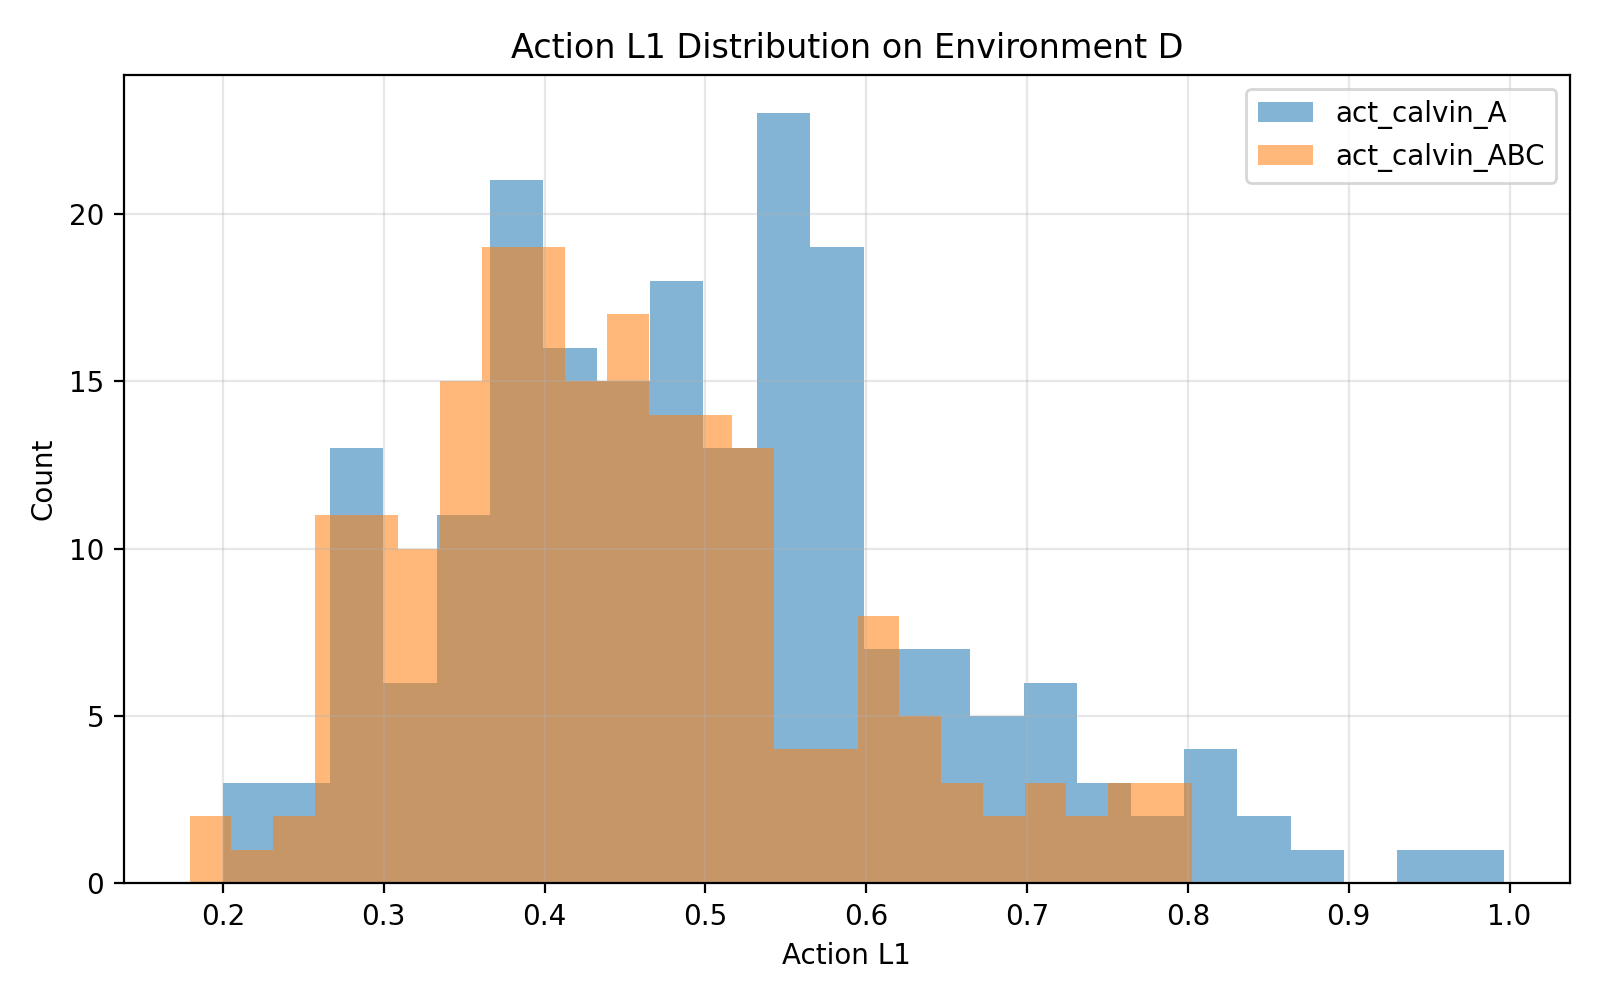
\includegraphics[width=\linewidth]{figures/action_l1_distribution.png}
\caption{D 环境动作误差分布}
\end{subfigure}
\caption{D 环境 zero-shot 评估可视化。越低表示动作预测越接近专家动作。}
\label{fig:eval_d}
\end{figure}

\section{现象分析}
\paragraph{多环境联合训练显著提升跨环境泛化。}
最终 D 环境 mean \actlone{} 中，\methodABC{} 为 0.4471，显著低于 \methodA{} 的 0.4963，下降约 9.9\%。这表明训练时引入 A/B/C 多环境视觉变化后，模型在面对未见过的 D 环境时能产生更接近专家的动作。该结果符合跨环境泛化的直觉：单环境 A-only 模型容易学习到与环境 A 外观绑定的视觉特征，而 ABC 联合训练迫使策略从多种背景和布局中提取更稳定的任务相关线索。

\paragraph{训练 loss 与泛化指标并不同步。}
在 30000-step 训练中，A-only 的训练 loss 仍然下降，但 validation \actlone{} 在 14000 step 后没有持续改善。类似地，ABC 在 27000 step 达到最好 validation \actlone{} 后，30000 step 反而回升到 0.4502。这说明更长训练不必然带来更好泛化，尤其在视觉模仿学习中，模型可能继续拟合训练域中的细节，却不提升验证域和测试域表现。因此，本实验使用 validation \actlone{} 而非最后一步选择 checkpoint 是必要的。

\paragraph{ACT 动作分块的鲁棒性与限制。}
ACT 的动作分块机制一次预测多个未来动作，能够在短时窗口内平滑控制输出，减少逐帧视觉噪声对动作的直接影响。在环境 D 的 visual distribution shift 下，这种机制有助于保持动作序列的连续性。但实验也显示，动作分块不能完全替代视觉泛化能力：A-only 即使使用 ACT，在 D 环境中仍明显落后于 ABC。这说明 ACT 的 temporal smoothing 与多环境视觉数据具有互补关系，前者提升短期动作一致性，后者提升跨环境表征鲁棒性。

\paragraph{30000-step 设置的选择。}
探索过程中比较了 25000 与 30000 steps。30000 steps 对 \methodABC{} 有小幅收益：D mean \actlone{} 从 0.4522 降至 0.4471；但对 \methodA{} 无收益，D mean \actlone{} 从 0.4918 升至 0.4963。综合题目关注的跨环境泛化对比，30000 steps 下 ABC 与 A-only 的差距更清晰，同时 validation-best 机制避免了直接使用过拟合的最后一步 checkpoint，因此本文采用 30000 steps 作为最终设置。

\section{结论}
本文完成了基于 LeRobot ACT 的跨环境泛化实验。结果表明，在相同网络结构与超参数下，A/B/C 多环境联合训练相比单环境 A-only 训练显著降低了环境 D 上的 zero-shot 动作误差。该现象说明，多环境数据能够提升视觉策略对环境外观变化的鲁棒性；ACT 的动作分块机制进一步提供了时序一致的动作输出，但其效果依赖于视觉表征是否足够环境不变。未来可进一步加入真实在线 rollout success rate、更多环境随机化和更长 horizon 的任务级评估。

\section*{外部链接}
\begin{itemize}
  \item GitHub 仓库：\url{https://github.com/Zhan-xing-pz/CS60003-HW3}
  \item 模型权重下载：\url{TODO: https://pan.baidu.com/s/<share-id>}
  \item 训练输出目录：\texttt{/data2/pz/homework/hw3/outputs}
\end{itemize}

\bibliographystyle{plain}
\bibliography{references}

\end{document}
